% evidential_calibration.tex - Calibration curve for evidential regression
% Data from Table 9.54: 100% empirical coverage at all confidence levels
% Shows severe over-calibration issue

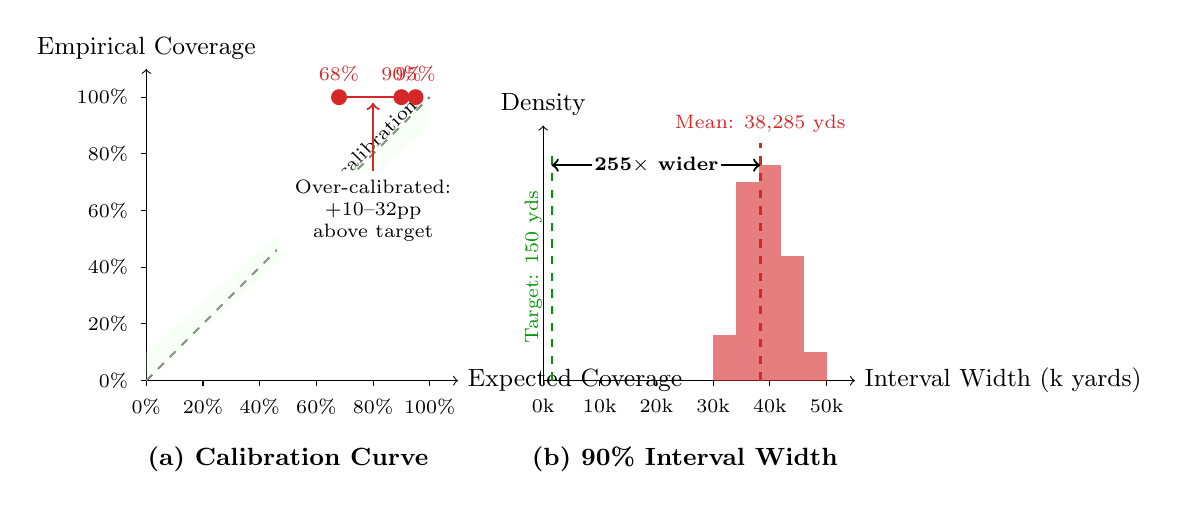
\begin{tikzpicture}[scale=0.72]
  % Define colors
  \definecolor{accent}{RGB}{31,119,180}
  \definecolor{overcal}{RGB}{214,39,40}  % Red for over-calibration

  % ============================================
  % LEFT PANEL: Calibration Curve
  % ============================================
  \begin{scope}
    % Axes
    \draw[->] (0,0) -- (5.5,0) node[right, font=\small] {Expected Coverage};
    \draw[->] (0,0) -- (0,5.5) node[above, font=\small] {Empirical Coverage};

    % Perfect calibration line (diagonal)
    \draw[dashed, black!60, thick] (0,0) -- (5,5);
    \node[font=\scriptsize, rotate=45, anchor=south] at (3.8, 3.6) {Perfect calibration};

    % Acceptable zone (±5%)
    \fill[green!10, opacity=0.3] (0,0) -- (5,4.5) -- (5,5) -- (0,0.5) -- cycle;

    % Data points (over-calibrated: all at 100%)
    \fill[overcal] (3.4, 5) circle (4pt);  % 68% expected → 100% actual
    \node[font=\scriptsize, overcal, anchor=south] at (3.4, 5.1) {68\%};

    \fill[overcal] (4.5, 5) circle (4pt);  % 90% expected → 100% actual
    \node[font=\scriptsize, overcal, anchor=south] at (4.5, 5.1) {90\%};

    \fill[overcal] (4.75, 5) circle (4pt);  % 95% expected → 100% actual
    \node[font=\scriptsize, overcal, anchor=south] at (4.75, 5.1) {95\%};

    % Connect points
    \draw[overcal, thick] (3.4, 5) -- (4.5, 5) -- (4.75, 5);

    % Axis ticks
    \foreach \x/\lab in {0/0, 1/20, 2/40, 3/60, 4/80, 5/100} {
      \draw (\x, -0.1) -- (\x, 0);
      \node[below, font=\scriptsize] at (\x, -0.15) {\lab\%};
    }
    \foreach \y/\lab in {0/0, 1/20, 2/40, 3/60, 4/80, 5/100} {
      \draw (-0.1, \y) -- (0, \y);
      \node[left, font=\scriptsize] at (-0.15, \y) {\lab\%};
    }

    % Over-calibration annotation
    \draw[<-, overcal, thick] (4.0, 4.9) -- (4.0, 3.5);
    \node[font=\scriptsize, text width=2.2cm, align=center, fill=white] at (4.0, 3.0) {Over-calibrated:\\+10--32pp above target};

    % Title
    \node[font=\small\bfseries, anchor=north] at (2.5, -1.0) {(a) Calibration Curve};
  \end{scope}

  % ============================================
  % RIGHT PANEL: Interval Width Distribution
  % ============================================
  \begin{scope}[xshift=7cm]
    % Axes
    \draw[->] (0,0) -- (5.5,0) node[right, font=\small] {Interval Width (k yards)};
    \draw[->] (0,0) -- (0,4.5) node[above, font=\small] {Density};

    % Histogram bars (extremely wide intervals centered at 38,285 yards)
    % Scale: 1 unit = 10,000 yards
    \fill[overcal, opacity=0.6] (3.0,0) rectangle (3.4, 0.8);
    \fill[overcal, opacity=0.6] (3.4,0) rectangle (3.8, 3.5);
    \fill[overcal, opacity=0.6] (3.8,0) rectangle (4.2, 3.8);
    \fill[overcal, opacity=0.6] (4.2,0) rectangle (4.6, 2.2);
    \fill[overcal, opacity=0.6] (4.6,0) rectangle (5.0, 0.5);

    % Mean marker
    \draw[overcal, very thick, dashed] (3.83, 0) -- (3.83, 4.2);
    \node[font=\scriptsize, overcal, anchor=south] at (3.83, 4.2) {Mean: 38,285 yds};

    % Target threshold
    \draw[green!60!black, thick, dashed] (0.15, 0) -- (0.15, 4.0);
    \node[font=\scriptsize, green!60!black, rotate=90, anchor=south] at (0.15, 2.0) {Target: 150 yds};

    % Comparison annotation
    \draw[<->, black, thick] (0.15, 3.8) -- (3.83, 3.8);
    \node[font=\scriptsize, fill=white, inner sep=1pt] at (2.0, 3.8) {\textbf{255$\times$ wider}};

    % Axis ticks
    \foreach \x/\lab in {0/0, 1/10, 2/20, 3/30, 4/40, 5/50} {
      \draw (\x, -0.1) -- (\x, 0);
      \node[below, font=\scriptsize] at (\x, -0.15) {\lab k};
    }

    % Title
    \node[font=\small\bfseries, anchor=north] at (2.5, -1.0) {(b) 90\% Interval Width};
  \end{scope}

\end{tikzpicture}
